\documentclass[conference]{IEEEtran}
% conference papers do not typically use \thanks and this command
% is locked out in conference mode. If really needed, such as for
% the acknowledgment of grants, issue a \IEEEoverridecommandlockouts
% after \documentclass
% \IEEEoverridecommandlockouts

\usepackage{color,graphicx}
\usepackage{cite}
\usepackage[cmex10]{amsmath}
%\usepackage{algorithm}
%\usepackage[tight,footnotesize]{subfigure}
\usepackage{subcaption}
\usepackage{url}
\usepackage{epsfig}
\usepackage{mathrsfs}
\usepackage{multirow}
\usepackage{textcomp}
\usepackage{rotating}
\usepackage{algpseudocode}
\usepackage{amssymb}
%\usepackage{slashbox}
\usepackage[colorlinks=true,citecolor=blue,pagebackref=true]{hyperref}


\definecolor{orange}{rgb}{1.0,0.3,0.0}
\definecolor{violet}{rgb}{0.75,0,1}
\definecolor{darkgreen}{rgb}{0,0.6,0}
\definecolor{cyan}{rgb}{0.2,0.7,0.7}
\definecolor{blueish}{rgb}{0.2,0.2,0.8}

\newcommand{\thunote}[1]{{\textcolor{cyan}{Thu: #1}}}
\newcommand{\xynote}[1]{{\textcolor{orange}{XW: #1}}}
\newcommand{\mdnote}[1]{{\textcolor{darkgreen}{Md: #1}}}
\newcommand{\ricardonote}[1]{{\textcolor{red}{Ricardo: #1}}}
\newcommand{\divyanote}[1]{{\textcolor{violet}{Divya: #1}}}

\newcommand{\myparagraph}[1]{\noindent {\bf #1}}

\newcommand{\tabincell}[2]{\begin{tabular}{@{}#1@{}}#2\end{tabular}}

% redefine enumerate env for closer spacing
% \renewenvironment{itemize}%
%   {\begin{list}{$\bullet$}%
%      {\topsep=0in\itemsep=0in\parsep=0in\partopsep=0in}%
%    }{\end{list}}

\begin{document}

\title{Grid-Aware Placement of Datacenters\\and Wind Farms
% \thanks{This work was partially supported by NSF grant XXX-YYYYYY %CSR-1117368
% and the Rutgers Green Computing Initiative.}
\vspace{-0.5in}
}

% Thu: Anonymity for double-blind review.
%
% \author{
% \IEEEauthorblockN{Xiaoying Wang} \IEEEauthorblockA{Department of
%   Computer \\
% Technology and Applications \\
% Qinghai University, China\\
% Email: wxy\_cta@qhu.edu.cn
% }
% \and
% \IEEEauthorblockN{Md E. Haque, \'I\~nigo Goiri, \\ Ricardo
% Bianchini, Thu D. Nguyen} \IEEEauthorblockA{Department of Computer Science\\
% Rutgers University, USA\\
% Email: \{mdhaque, goiri, ricardob, \\
% tdnguyen\}@cs.rutgers.edu
% }
% \and
% \IEEEauthorblockN{Divya Kurthakoti Chandrashekhara}
% \IEEEauthorblockA{Siemens Corporate Research, USA\\
% Email: div.s.sya@gmail.com
% }
% }


% \IEEEpubid{978‐1‐4799‐0623‐9/13/\$31.00~\copyright~2013 IEEE}
% \IEEEpubid{978‐1‐4799‐0623‐9/13/\$31.00~\copyright~2013 IEEE}
%\IEEEpubid{\makebox[\columnwidth]{978‐1‐4799‐0623‐9/13/\$31.00~\copyright~2013 IEEE \hfill} \hspace{\columnsep}\makebox[\columnwidth]{ }}

% \CopyrightYear{2013}
% \copyrightdata{978‐1‐4799‐0623‐9/13/\$31.00~\copyright~2013 IEEE}

%\IEEEpubidadjcol

\date{}

\maketitle

\begin{abstract}

  Datacenters consume a massive amount of energy, and this consumption is increasing rapidly.  As new datacenters are built, environmentally conscious operators are seeking to mitigate their environmental impact by building offsetting renewable power plants.  These renewable power plants may or may not be co-located with datacenters.  While a number of research efforts have looked at the optimal placement of new datacenters and renewable power plants, they have mostly neglect the impact on the electricity transmission grid.  With rapidly increasing penetration of such ``renewable powered datacenters,'' it is becoming imperative to study their impact on the tranmission grid.  In this paper, we show that considerations of the impact on the transmission grid when placing new datacenters and renewable power plants can be mutually beneficial to both grid operators and datacenter owners.  Specifically, locating datacenters and renewable power plants at strategic places in the grid could help to minimize (i) overloading of transmission lines, (ii) grid voltage variations outside the acceptable range, and (iii) system losses.  We develop an optimization framework for placing a new datacenter and wind farm, and use it in a case study to show that considering transmission losses can lead to different placement and lower overall cost.  Interestingly, co-locating the datacenter and wind farm does not always lead to lowest impact on the transmission grid and lowest overall cost.  Thus, we conclude that optimal placement of new datacenters and renewable power plant can only be achieved by jointly considering the impact of location on the costs for the datacenter owners as well as for the grid operators.

\end{abstract}


%%% Local Variables:
%%% mode: latex
%%% TeX-master: "paper"
%%% End:

\section{Introduction}
\label{sec:intro}

Datacenters are being constructed at a rapid pace as computing is increasingly moving to the cloud (e.g., \cite{RM14DCGrowth}).  As new datacenters are built, some companies are seeking to mitigate the environmental impact of their massive energy consumption by also building offsetting renewable power plants (e.g.,~\cite{GoogleGreen,Apple13,McGrawHill11}).  Both the new datacenters and the accompanying renewable power plants can pose challenges to the electricity grid.  Specifically, a large datacenter can require upward of 100MW of power, presenting a significant load to the grid.  Since adding transmission capacity to the grid takes a long time (typically 7 to 10 years) and is extremely expensive \cite{interconnection2010survey}, attaching new large datacenters and renewable power plants to the grid can lead to increased overloading of transmission lines, grid voltage variations outside the acceptable range, and transmission system losses.  Thus, the increasing penetration of such {\em renewable powered datacenters}\footnote{Note that we are calling a datacenter together with an offsetting renewable power plant a ``renewable powered datacenter'' for brevity, even though the two may {\em not} be physically co-located.} makes it imperative to study their impact on the transmission grid.

Researchers have studied the placement of new datacenters since they are expensive to build and operate, and parts of the construction and operation costs are location-dependent~\cite{Goiri11place,Dalger05,Boley09,larumbe2012optimal,berral2014building}.  However, these studies have not considered the impact of new datacenters on the grid.  Others have studied whether the renewable power plants should be co-located with the datacenters\cite{Ren12MASCOTS}, and have considered transmission loss when the datacenter and the renewable power plant were physically distributed.  However, only a fixed loss percentage was assumed.

In this paper, we first show that the placement of a large renewable powered datacenter can significantly impact the transmission grid, and that careful placement can be beneficial to both the grid operators and datacenter owners.  Specifically, we study the impact of placing a datacenter and an offsetting wind farm within a real world transmission system of the New England Independent System Operator (ISO) spanning most of North Eastern region of United States and some parts of Canada.  We use simulation to show that datacenters/renewable power plants located at strategic places in the grid could help minimize i) overloading of transmission lines; ii) grid voltage variations outside the acceptable range; iii) system losses.


% Furthermore, grid losses are on of the largest expenses for the power system operators \cite{de2014investigation}. EIA (U.S. Energy Information Administration) \cite{EIA} has estimated that the electricity transmission and distribution losses all over the U.S. is about 6\% of the electricity that is transmitted and distributed each year (averaged from 1990 to 2012). Thus, reduction of these losses for the grid can greatly affect the total operational costs.

% As reported recently, the energy consumption of datacenters keeps growing while more and more enterprises and organizations are building their own datacenters\cite{urgaonkar2011optimal,Koomey2011}. The increasing speed of the datacenter energy consumption is approximately 10-12\% per year recently \cite{ghatikar2014demand}. The carbon emission and environment pollution issues attract insights of seeking for clean energy resources. Many IT companies such as Google\cite{GoogleGreen}, Apple\cite{Apple13}, and McGrawHill\cite{McGrawHill11} are trying to build their datacenters together with renewable energy power plants.


% Usually, generation of sustainable energy like solar and wind will be closely related to the weather condition at certain locations. As far as we know, there might be different choices for building the datacenter and the power plants. Both on-site and off-site generation are possible approaches \cite {Goiri13}. By grid-centric approaches, the renewable energy will be generated at locations with sufficient renewable sources and pumped into the grid. On the other hand, co-location and self-generation approaches sit the datacenter and the power plant at the same location to facilitate management and avoid long-distance losses. Since it seems no approach is perfect, we argue that companies essentially expect benefits from the investments by building up datacenters and green power plants. However, since the renewable energy generation is mostly intermittent and sometimes might bring great penetration current into the electric grid, the capacity should be carefully planned and will be limited from the perspective of grid operators. For example, some tiny failures may make an area of grid system completely out of power \cite{nytimes2014}.

% Since datacenters are becoming quite large loads for the electric grid, they are supposed to have a significant impact on the operation of power grid \cite{haowang2014grid}. Large datacenter loads might increase the grid load and also lead to significant load variability of the electricity system. Especially, the emergence of the renewable energy sources with intermittent nature brings fluctuations onto the electricity networks. Furthermore, grid losses are on of the largest expenses for the power system operators \cite{de2014investigation}. EIA (U.S. Energy Information Administration) \cite{EIA} has estimated that the electricity transmission and distribution losses all over the U.S. is about 6\% of the electricity that is transmitted and distributed each year (averaged from 1990 to 2012). Thus, reduction of these losses for the grid can greatly affect the total operational costs.

% In this case, companies who want to build datacenters with either on-site or off-site renewable energy plants have to get the permission from the grid operators first in order to reduce the unexpected influence to the grid operation. Since the grid losses will also finally turn into expenses for end-users, service providers may want to collaborate with grid operators to minimize the overall cost when planning locations and capacity for the datacenters. In the current literature, datacenter placement issues have been mentioned in some prior work\cite{Goiri11place,Dalger05,Boley09,larumbe2012optimal}, and there are also some research focused on the capacity planning of green datacenters \cite{Le10,berral2014building}. Nevertheless, these work hasn't considered the impact of datacenter placement on the grid itself, which might also lead to comparable costs as other costs for datacenters.

Next, having shown that the placement of new renewable powered datacenters can significantly impact the transmission system, we proceed to develop an optimization framework for minimizing the total cost of building and operating new datacenters.  Similar to previous works in this area, our framework considers the various capital costs (e.g., land and construction costs) and operational costs of building and operating a new renewable powered datacenter.\footnote{Note that we are not proposing a new method for the placement of renewable power plants (specifically wind farms in our study).  Our cost models are likely simplistic compared to existing techniques for finding good locations for new wind farms.  Rather, the point of our work is that costs for the placement of a new datacenter, renewable power plant, {\em and} their impact on the transmission grid should be studied together.}
  Unique to this work, however, is the added consideration of the cost of system loss in the transmission grid, as well as constraints of avoiding transmission line overloading and unacceptable voltage variations.

Finally, we use our optimization framework in a case study to demonstrate the potential benefits of our placement approach.  Specifically, we again study the placement of a new datacenter and an offsetting wind farm in the New England ISO system.  \thunote{Need to give a couple of sentences here to summarize our results.} Results of our case studies illustrate that by jointly considering the placement of the datacenter and the wind farm, the total cost will be reduced compared to other strategies, including the cost of system losses in the electric grid.

% In this paper, we attempt to set up a different point of view, by combining the consideration for cloud service providers and energy companies together and aiming at the minimization of the overall cost for both. First, we investigate the impact of datacenter placement and its importance to the grid by studying a region of grid network. We pay special attention to the datacenter size, datacenter locations and the variation of renewable power generations. Second, we formulate the optimization framework, which incorporates the costs of datacenters, renewable power plants and power grid into one objective. We also try to solve it under necessary constraints by using several different approaches. Then we conduct a case study in the New England area of the United States, by sitting and provisioning datacenters and power plants at different locations, with the purpose of minimizing the overall cost. Results show that grid losses can have remarkable impact on the decision of selecting best locations for green datacenters. Furthermore, the co-location choices by sitting the datacenter and green plants together don't show advantages despite of the reduced line cost and distribution cost, which is not that intuitive as prior work thought.

\myparagraph{Contributions.} Our main contributions include: (i) demonstrating the potential impact of renewable powered datacenter placement on a transmission system, (ii) proposing an optimization framework for the smart placement of both datacenters and renewable power plants in the power grid network, and (iii) exploring the potential benefit of the placement framework in a realistic case study.

% To the extent of our knowledge, there is no previous work considering the jointly placement issues of datacenters and green power plants while caring about the grid operational costs together. The remainder of the paper is organized as follows. Section \ref{sec:quantify} first quantifies the potential of datacenters together with wind farms by placing them into different buses of the grid network system. In Section \ref{sec:framework}, we describe the optimization framework in detail, showing the integration of various parameters of the entire problem. Section \ref{sec:eval} evaluates the costs and illustrates breakdown of the total cost by different kinds of strategies. In Section \ref{sec:related}, we present some prior work related to this paper. Finally, the conclusion is given in Section \ref{sec:conclusion}.


%We discuss each of these in detail as following:(1) \textbf{The potential of datacenter placement on grid.} (2) \textbf{Jointly placement of datacenters and renewable energy power plants.}


%%% Local Variables:
%%% mode: latex
%%% TeX-master: "paper"
%%% End:

\section{Impact of Datacenter Placement on the Grid}
\label{sec:quantify}
%PLEASE INCLUDE THIS/APPROPRIATELY EDITED FORM OF THIS TEXT IN INTRODUCTION%%%%
%Today many datacenters are being powered by renewable energy source like wind and solar. There are two choices of locating the datacenters i) near the wind or solar farm, what we refer to as co-location in the paper or ii) away from the renewable energy source (power is transmitted over long distance transmission lines). This paper answers the questions i) how do we decide which of the two is better and ii) how do we plan the datacenter location if we have multiple choices. In order to decide which one of these choices are better we need to define a comprehensive metric. In this paper we will first define these metrics and justify by considering a realistic scenario of placing datacenter in the New England system. Later, we provide a planning methodology that can be used to determine the datacenter location in any electric grid with wind or solar power. Finally, we propose an optimization algorithm that can be used to determine the best datacenter location under a given set of constraints.
%%%%%%%

In this section, we first discuss different ways that the placement of renewable powered datacenters can impact the power grid.  We then describe a simulation system that we have built to quantitatively explore this impact.  Finally, we present some results to show that it is important to consider grid impacts when locating new renewable powered datacenters.

% Planning optimal datacenter location, requires comprehensive metric definition. Most of the studies carried out so far neglect the impact of renewable powered datacenters on the transmission grid. When the penetration of renewable powered datacenters was small, the impact of these on the transmission grid was insignificant. However, with several large datacenter companies opting for renewable energy source it becomes imperative to study their impact on the transmission grid.

\subsection{Potential Impacts}

The rapidly increasing penetration of large renewable powered datacenters can potentially impact the power grid in several ways.

\subsubsection{Overloading of transmission lines}
Transmission lines (also referred to as ``branches'') are used to transport power from the large generators to the load. The power carrying capacity of each line is limited to protect the line from overheating, mainly due to the line resistive losses, i.e., $I^{2}R$, where $I$ is the current flowing through the line and $R$ is the resistance of the line.

A transmission line typically has two ratings: short term and long term capacity rating. During certain wind and system load (including datacenter load) conditions, some of the transmission lines could get overloaded. If this happens during the normal operation of the grid then one of the following will be done: i) if an electronic power flow controller is available then it is used to control the power flow through the overloaded line; or ii) in extreme situations, the overloaded line is disconnected which may result in power supply interruption to the loads.

If major transmission lines are getting overloaded quite often annually then new lines are planned and built.  As already mentioned, this solution is very expensive and takes a long time. The need for such expensive grid retrofits may be minimized by planning the location of large new generators such as wind farms and large new loads such as datacenters.

\subsubsection{Voltage variations}
The voltage magnitude varies in the electric grid, and needs to be maintained within a narrow range (for example +/- 5\% of nominal) to avoid damaging sensitive electronic loads.  Unfortunately, there are times when changes in the power output of renewable power plants can cause the voltage to vary beyond the acceptable limits. Such over/under voltage problems can be mitigated by appropriately locating new renewable powered datacenters.

\subsubsection{System losses}
Historically, the electric grid was designed to have large central generating stations that are located far away from the load centers. The power from these central sources would be transmitted to the load centers over transmission lines. While designing such a grid, the generator location and the transmission line voltage level as well as the path would be optimized to minimize the line losses.  With increasing penetration of renewable power, however, this scenario has changed: the generation sources are distributed and may be located near the load centers.  Yet, we still use the existing transmission lines that were planned and built about 50 years ago or earlier.  This may result in higher line losses and sub-optimal power transmission between generation sources and loads. Since we cannot re-design the entire electric grid to minimize line losses, we need to leverage the flexibility we have in locating new sources and loads, i.e., renewable powered datacenters in our specific case.


\subsection{Simulation study}
In order to quantitatively study the impact of renewable powered datacenter location in a power grid, we consider the New England ISO transmission network. We choose this system for the following reasons:

{\em Wind power expansion in New England:} System studies carried out by the New England ISO show that there is a potential for integrating up to 12 Giga-Watts of wind power in this region.  This enormous potential for wind power makes the region an interesting destination for datacenters powered by wind farms.

{\em Transmission network upgrades:} A study carried out by the New England ISO shows that they could potentially integrate wind resources to meet up to 24\% of the region's total annual electric energy needs in 2020 if the system includes transmission
upgrades. If these transmission upgrades can be limited then the development of new wind farms becomes more economical.

{\em Positive impacts of wind power in New England ISO:} Introducing large amounts of low-marginal-cost wind generation tends to depress the spot price and reduce the price differential for bulk power between day and night. Also the study results demonstrated that there was only a relatively small increase in the use of existing pumped-storage hydro power for large wind penetrations, largely because the flexible natural-gas-fired generation fleet provided most of the system balancing.

We will show in our study, that within the New England ISO, the wind power penetration can be increased much more cost effectively by strategically locating the datacenter. Intuitively, it may appear that co-locating datacenter loads and wind farms would solve the problem of building new transmission lines, limit the voltage variation and also minimize losses. However, our study shows that this is not indeed true and co-locating wind farm and datacenter may not be the optimal solution always.

Before we carry out the case studies, we will describe the approximations we made and the models we used for each sub-system we considered in our study.
%\thunote{Divya, I think we need to explain why we are adding wind farms and datacenters to the model.  Also, we need to briefly say how we figured out the bus-to-physical-location mapping.  Finally, we also need to briefly talk about the assumed load on the grid.}

{\em New England transmission system model:}
For our study we considered a widely used  \cite{bills1970line} model of the New England transmission network. A single line diagram of this test system is shown in Figure~\ref{fig:newengland}. As shown in the figure, the model lumps all the generators, loads and transmission lines in the New England ISO region to 10 generators, 19 loads and 46 lines and transformers. The 10 generator buses are numbered from 30-39 in Figure~\ref{fig:newengland}. Specifically, bus 39 represents the aggregation of a large number of generators interconnected to rest of US/Canada.  This model includes load data for periods of low and high loads.

%%%
\begin{figure}[ht]
\centering
\includegraphics[width=1\columnwidth]{img/newEngland.jpg}
\caption{New England 39 bus test system}
\label{fig:newengland}
\end{figure}
%%%

{\em Datacenter model:} Since the model of the New England system was created, large datacenters have been added to the region.  To account for this added new load, we collected information on datacenters in the area from~\cite{DCmap}.  Then, using a mapping of the buses in the model to geographic locations, we aggregate all the datacenters in the New England ISO region into six datacenters, each representing datacenters in a state, and placed each aggregated datacenter on a bus appropriate for that state.  We estimate the size of each ``aggregated'' datacenter as 
$L_i=(n_i* 1.45 * 9.8GW)/1278$, where $L_i$ is the aggregated load of the $i$th state, $n_i$ is the number of datacenters in that state, 9.8GW is the upper bound of total electricity used by US datacenters in 2010 \cite{Koomey2011}, 1.45 is a rough estimate of growth in datacenter electricity consumption from 2010 to 2014 (using information from \cite{Koomey2011}), 
and 1278 is the total number of datacenters in the US as reported in \cite{DCmap}.
% However, according to \cite{Koomey2011}, for the summarized load of datacenters, there is an increase of 56\% from 2005-2010. Hence, we are assuming the increasing percentage from 2010-2014 is 56\%*0.8=45\%, and after adjustment we are using $L'_i=1.45L_i$ as the datacenter load for the target grid system.
Table~\ref{tab:dc_setting} shows the placement of these aggregated datacenters and their sizes.

\begin{table}[ht]
\begin{center}
\caption{Background datacenter load and location settings}
\begin{tabular}{|l|l|p{30pt}|p{50pt}|p{30pt}|}
\hline
DC No. & State & Number of DCs & Estimated  aggregate size (MW) & Mapped Bus No.\\
\hline
DC1 & Connecticut & 12 &133.43 & 6\\
DC2 & Maine & 3 &33.36 & 29 \\
DC3 & Vermont & 4 &44.48 & 25 \\
DC4 & Rhode Island & 3 &33.36 & 20\\
DC5 & New Hampshire & 4& 44.48 & 16\\
DC6 & Massachusetts & 27& 300.21 & 4 \\
\hline

\end{tabular}
   \vspace{.05in}
\label{tab:dc_setting}
\end{center}
\end{table}


{\em Wind farm model:}  We have similarly added wind farms to the model to represent recent penetration of wind energy.  Specifically, lumped models of several wind farms within geographical regions have been connected to bus 18, 28, 36, 37 and 38. 
The locations and capacity settings of the five wind farms are presented in Table~\ref{tab:wf_setting}. We assume that each farm can be represented by $n$ identical wind turbines, where $n$ is equal to the total farm rated capacity divided by the individual wind turbine rating. This approximation does not change any of our results because we are interested in studying the global impact of wind farm powered datacenters on the electric grid. Also, since most of the wind turbines in this region are GE 1.5MW machines, we use the 
wind speed versus power characteristics of this turbine model\cite{lei2006modeling}.
For this particular turbine model, the cut-in wind speed, i.e., the wind speed at which the turbine starts producing power, is 5m/s and the cut-off wind speed is 25m/s, beyond which the turbine will be shut down for safety reasons. The wind turbine produces rated output that grows linearly from near 0MW to 1.2MW for wind speeds from 6m/s to 10m/s, then more slowly to reach the top rated output of 1.5MW between wind speeds of 13-25m/s.  We assume that wind farms are not provisioned with energy storage capacity.

% \red{Note that the wind farms don't have energy storage equipped and the wind energy will be directly penetrated into the grid. Our focus is to show that in any electric grid it is important to consider the transmission grid constraints while deciding the data center location. Also we believe that optimally located data center can replace energy storage functionality to a certain extent. For example, the transmission line congestion can be reduced by appropriately placing the energy storage. However, a cost effective and optimal manner to do it is to use the algorithm we have proposed in this paper to locate the data center. Another reason we are not considering energy storage is because there are diverse types of energy storage and not all of them are cost effective. Also we believe that the topic of cost effective and practically viable energy storage is an independent research topic. A comprehensive study has been presented in \cite{rosen2011energy}.}

%  From Figure~\ref{fig:windcurve} we can see that the cut-in wind speed,
% %%%
% \begin{figure}[ht]
% \centering
% 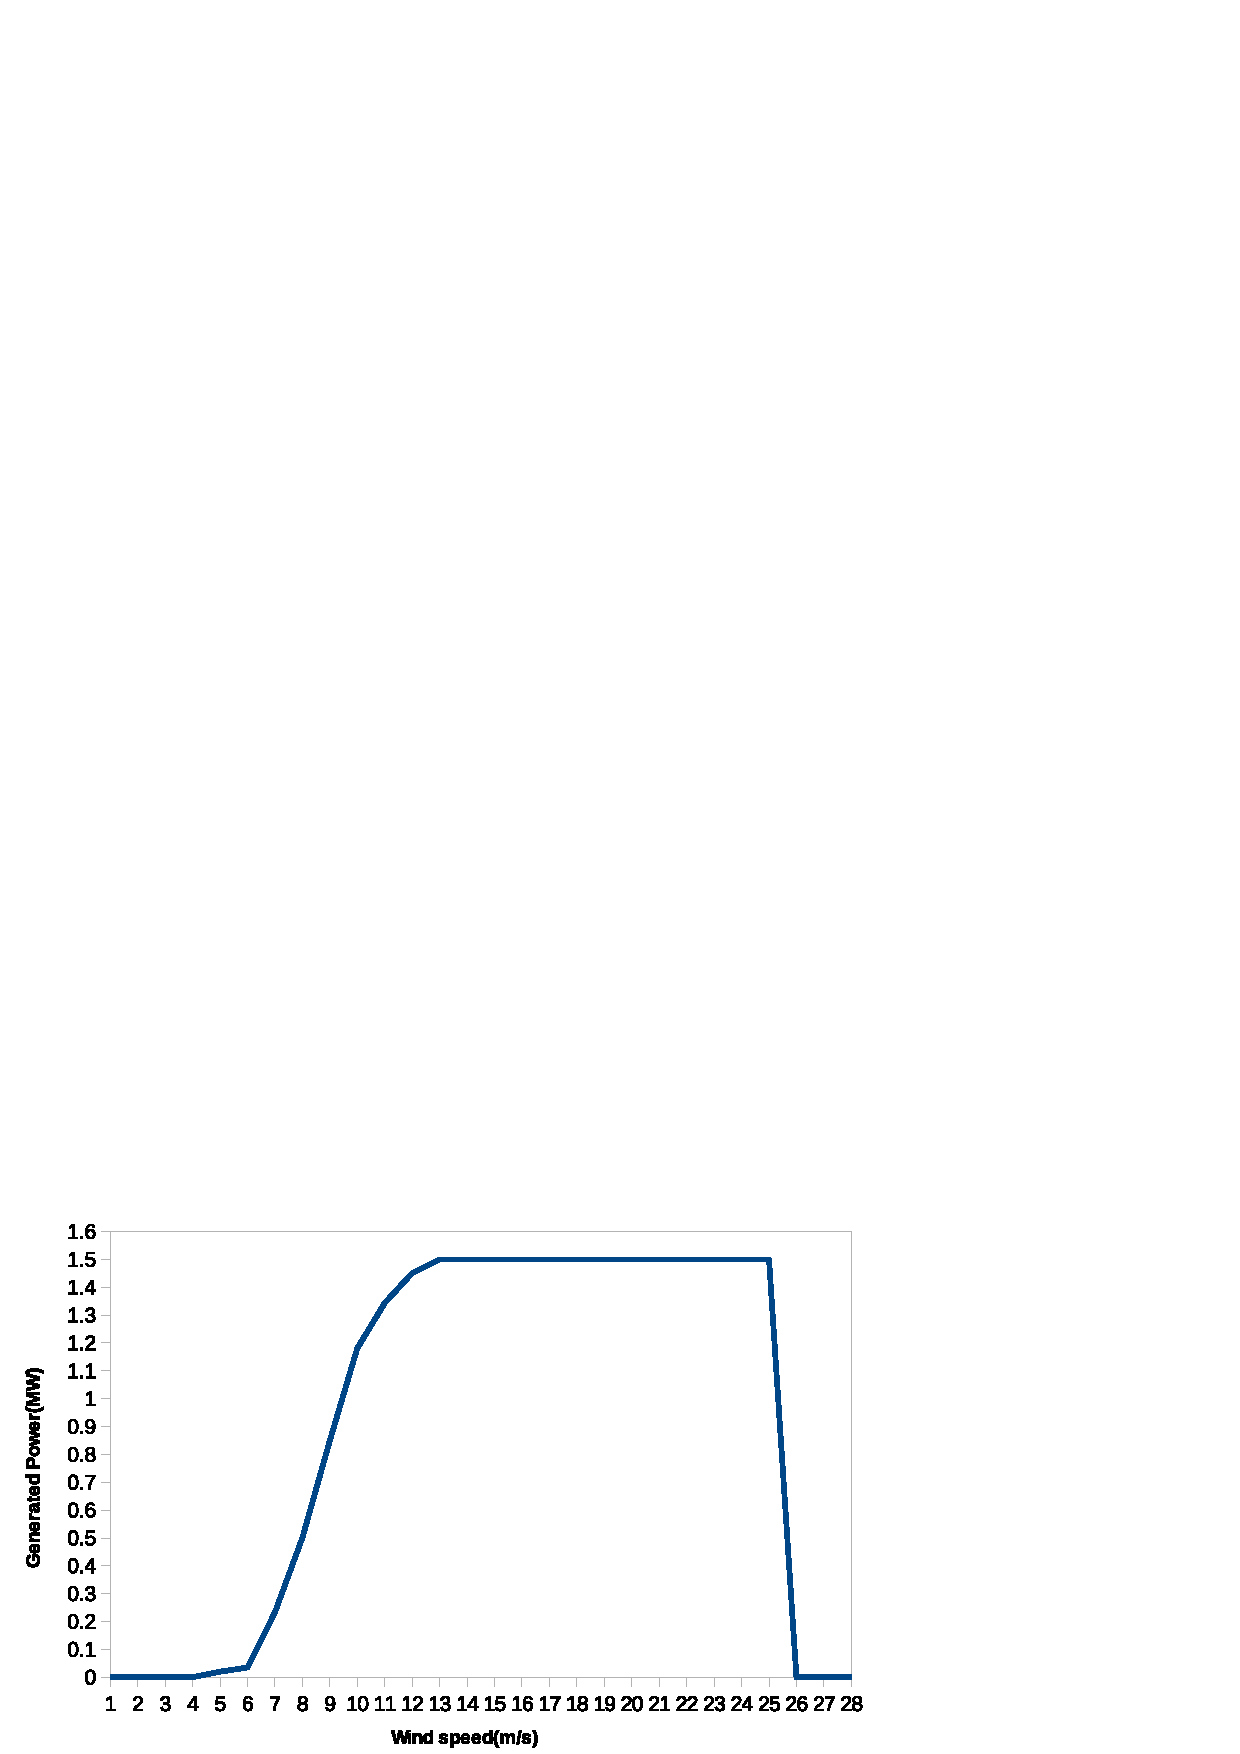
\includegraphics[width=1\columnwidth]{img/wind_curve.pdf}
% \caption{Power curve of the GE 1.5MW wind turbine}
% \label{fig:windcurve}
% \end{figure}
% %%%


\begin{table}[ht]
\begin{center}
\caption{Background wind farm settings}
\begin{tabular}{|l|l|c|c|}
\hline
WF No. & Bus No. & State & Capacity(MW) \\
\hline
WF1 & 18& New Hampshire & 100\\
WF2 & 28& Maine & 90 \\
WF3 & 36& Vermont & 90  \\
WF4 & 37& Maine & 90\\
WF5 & 38& Massachusetts & 90\\
\hline

\end{tabular}
   \vspace{.05in}
\label{tab:wf_setting}
\end{center}
\end{table}

\subsection{Case study}
\label{sec:casestudy}

We use the above ``modified'' New England model to study the impact of
connecting a new datacenter to an electric transmission system.
Specifically, we assess the impact using the three metrics described
earlier for three case studies:

{\bf Case 1:} The base modified New England system.

{\bf Case 2:} The modified New England system with one additional
200MW datacenter co-located with one of the wind farms in
Table~\ref{tab:wf_setting}.

3) The modified New England system with one additional 200MW
datacenter connected to a bus away from all wind farms in 
Table~\ref{tab:wf_setting}.

We compute the power flows through the transmission lines, the bus
voltages, and the system losses by solving a set of power flow
equations that model the power balance in a transmission system (i.e.,
net load + losses = total generation).
Within an electric grid the power
can be easily measured at the loads and at generators. Also, some
generators have the capability to regulate the voltage at a bus at a
constant preset reference value. The power flow equations are used to
calculate the bus voltages (magnitude and angle), for a given network
and a set of load and generation powers. The power flow equations for a
generic $n$ bus network with $k$ branches are:

\begin{equation}
P_{i} = \Sigma_{j=1}^{n}(|Y_{ij}||V_{i}||V_{j}|cos(\theta_{ij}+\delta_{j}-\delta_{i})
\end{equation}
\begin{equation}
Q_{i} = -\Sigma_{j=1}^{n}(|Y_{ij}||V_{i}||V_{j}|sin(\theta_{ij}+\delta_{j}-\delta_{i})
\end{equation}

\noindent where $P_{i}$ and $Q_{i}$ are real and reactive powers at
the $i^{th}$ bus; $|V_{i}|\angle \delta_{i}$ are the voltage magnitude
and angle at the the $i^{th}$ bus; $|Y_{ij}|\angle \theta_{ij}$ is
the admittance of the branch between $i^{th}$ and $j^{th}$ bus.  For a
given pair of powers $P_{i}$ and $Q_{i}$ at the $i^{th}$ load bus, the above
power flow equations are used to solve for the voltage magnitude and
angle at the $i^{th}$ bus. Since the above equations, i.e., real and
reactive powers are non-linear function of voltage they are solved
iteratively using Newton Raphson method. Once the bus voltages are
calculated the line flows and system losses are
computed.

\subsection{Results and discussion}
%I need only the following results for each case (Case1, Case2 and Case 3):
%1. a table containing system losses for each case (total loss its only one number for each case)
%2. any line capacity violations (line number)
%3. voltage violations if any (bus number)
%%%

Here, with respect to the three cases mentioned above, we calculate
line power flows, bus voltages and the value of system losses
respectively by conducting simulation experiments, and then discuss
the results under the condition of different placement choices for the
datacenter.

First, we simulate the three cases under peak system load (6,885MW in
total) to explore differences in line overloading.  The wind speed is
set to LOW (4-6m/s), implying that the power generated by the wind
farms is nearly zero (less than 2.3\% of the rated capacity).  For
Case 2, the datacenter is connected to bus 18 (and so is co-located
with wind farm WF1), and for Case 3, the datacenter is connected to
bus 10 (away from all wind farms).  Table \ref{tab:results-linevio}
shows the number of line overloads in the system.  These results
highlight that different placements of the additional datacenter can
result in line overloading.  Although there are only a few cases of
line overload in our experiments, annually the number of overloads and
their durations will depend on the frequency and duration of
occurrences of a particular wind speed and load condition. If it is
too frequent or more persistent, then the overloads could be a serious
problem and might require building new transmission lines. According
to \cite{interconnection2010survey}, the estimated cost of building
new transmission lines of 345kV voltage level is about \$2.5
Million/mile, which is very expensive with total costs in the billions
of dollars. Hence, it's important to choose the right place for
datacenters in order to mitigate line overloading occurrences.

\begin{table}[ht]
\begin{center}
\caption{Results of overloaded lines}
\begin{tabular}{|c|c|c|}
\hline
Case No. & \# of overloaded lines & List of overloaded lines \\
\hline
1 & 0 & None\\
2 & 1 &  bus 4 - bus 5 \\
3 & 0 & None \\

\hline

\end{tabular}
%   \vspace{.05in}
\label{tab:results-linevio}
\end{center}
\end{table}

Next, we investigate unacceptable voltage variations in the
transmission system, as shown in Table \ref{tab:results-volvio}. Here,
the wind speed setting is MEDIUM (8-10m/s), which means the generated
power of each wind turbine will be 33.3\%-78.7\% of its rated
capacity.  For Case 2 the datacenter is located at bus 38 (co-located
with wind farm WF5), and for Case 3 the datacenter is located at bus
25 (away from all wind farms). The acceptable voltage range of a bus
is set to [0.95p.u.,1.05p.u.]. It can be observed under these
conditions condition, there is already an unacceptable voltage
deviation in the base modified New England system.  Case 2 increases
the number of unacceptable voltage deviations to four.  In contrast,
Case 3 has no unacceptable voltage deviations.  These results show
that unacceptable voltage variations can be mitigated by carefully
choosing the place for the new datacenter.

\begin{table}[ht]
\begin{center}
\caption{Results of voltage variations}
\begin{tabular}{|c|p{1in}|p{1in}|}
\hline
Case No. & \# of buses with voltage deviation & List of buses with voltage deviation  \\
\hline
1 & 1 & bus25\\
\hline
2 & 4 & \tabincell{c}{bus25\\bus26\\bus28\\bus29}\\
\hline
3 & 0 & None \\

\hline

\end{tabular}
\label{tab:results-volvio}
\end{center}
%\vspace{-0.25in}
\end{table}

Finally, we compare the total system losses for the three cases under
three different wind speeds: LOW, MEDIUM, and HIGH.  The results are
shown in Figure~\ref{fig:loss-cases}.  Here, the load is set to normal
(6,254MW in total).  LOW and MEDIUM wind speeds are as before.  HIGH
wind speed corresponds to 11m/s, such that the output power of the
wind turbine is very close to its rated capacity. For example, a 100MW
wind farm would be generating at least 89.6MW of power under HIGH wind
speed.  The datacenter is located at bus 18 (co-located with wind farm
WF1) for Case 2, and at bus 10 (away from all wind farms) for Case 3.

\begin{figure}[hb]
\centering
\includegraphics[width=1\columnwidth]{img/loss3cases.pdf}
\caption{Results of system losses}% \red{with 95\% confidence intervals}}
\label{fig:loss-cases}
\end{figure}

Results in Figure~\ref{fig:loss-cases} show that the co-location case
(Case 2) could lead to greater loss than Case 1 and Case 3. For
example, at MEDIUM wind speed, the system loss for Case 3 is about 6\%
less than Case 2, which illustrates system loss can be reduced by
careful placement of the datacenter, and co-location with a wind farm
is not necessarily the best choice.

Note that even though we have provided only one set of results for a
specific set of conditions, we have simulated different wind speeds and
load conditions.  The results consistently show that the placement of
a new datacenter can significantly impact transmission system losses,
and that co-location with a wind farm is often not the best placement
strategy.
%% We found that in general the system loss magnitude
%% could change. However, in most cases we saw that co-location is not
%% the optimal choice for minimum system loss. In Section
%% \ref{sec:framework} we will describe a method for determining the
%% datacenter location that will correspond to minimal system loss
%% annually and will cover all the wind speed and system load conditions.


%%% Local Variables:
%%% mode: latex
%%% TeX-master: "paper"
%%% End:

\section{Framework for smart placement}
\label{sec:framework}

The previous section highlights that placing data centers and wind
farms has obvious impact on the grid trasmission network system. Thus,
when a service provider is looking for best locations to estabish a
network of green data centers, the grid operational cost should also
be included as one of the most important factors into
consideration. Another observation is that co-location of the green
data center and the green energy plant seems not always be the best
choice. In this case, we try to study how to seek the best locations
for both the data center and the green energy plant, which are
designed to be connected to the same grid network.

By grid-aware placement, we attempt to efficiently select a set of locations for one or more data centers to support a given amount of computational power, as well as one or more green power plants (e.g. solar, wind or others) to provide a given power capacity. The main goal is to minimize the overall cost for data centers, green power plants and also the grid network operation. The next subsections defines some important parameters in the selection procedure. Then, the cost model and the entire optimization problem will be formulated and described.

\subsection{Parameters for the placement framework}

Table \ref{tab:par_setting} gives all of the parameters defined in our framework.  These parameters relate to costs, revenue and losses over different geographical locations. We generally classify them into three categories: data-center-related, renewable-related and grid-related.

\subsubsection{Data-center-related costs} Given a target capacity of how large a data center is planned to build, we can calculate the capital cost first. The capital cost of a data center at location $l$, denoted as $DC\_CAPcost(l)$, can be broken down into land cost ($DC\_landCost(l)$), building cost ($DC\_buildingCost(l)$) and hardware cost($DC\_hwCost(l)$). Land cost can be computed by land price at that location and the accommodated data center capacity. Building cost depends on the maximum capacity of the data center, too. Hardware cost contains both server cost and switch cost, which can be computed given the total capacity of the data center. Besides, hardware cost also includes costs for building lines connecting the data center to the Internet backbone and the transmission grid, denoted as $costLineNet(l)$ and $costLineGrid(l)$ here respectively. We assume them independent of the data center size, but dependent on the location $l$ of the data center.

Besides capital costs, operating and managing a data center also incurs operational cost, including costs for using the network bandwidth and the electricity from the power grid. We denote them as $DC\_netCost(l)$ and $DC\_energyCost(l)$ respectively, which both depend on the location $l$ of the data center. Furthermore, the energy cost for the data center is also related to the varying demands of the data center workload over different time period, denoted as $demand(l,t)$ hereafter.

\subsubsection{Renewable-related costs} The costs for building and running a renewable power plant also include capital costs and operation costs. The capital cost of a type $r$ plant at location $l$, denoted as $RE\_CAPcost(l,r)$, can be broken down into land cost ($RE\_landCost(l,r)$), building cost ($RE\_buildCost(l,r)$) and line cost ($costLineNet(l)$) for connecting to the transmission grid. Specially, if we are also building a data center in the same location, the connection line to the grid could be shared by the plant, and in this case the line cost could be saved. Similarly, the land cost for renewable power plant depends on the needed area and the land price at that location. The building cost mainly depends on the desired capacity of the plant.

Regarding operational costs, we assume that the human and labor costs for maintenance and operation are same over different locations. Thus, by operating the renewable power plant, we only consider the possible revenue it could bring by generating electricity power and transmitting power to the grid. Here, we regard the revenue as a negative cost for the power plant, denoted as $RE\_OPrev(l,r)$, which is closely related to the power generation efficiency at the location and the energy selling price there.

\subsubsection{Grid-related costs} When connecting the data centers and the renewable energy plants to the utility grid, we are adding both generation and consumption components into the network. This will change the power flow of the whole network, and thus the total losses of the transmission network will be different. Thus, the transmission loss ($transLoss(t)$) will be affected by the generating and consuming power amount of data centers and renewable plants, and also the buses they are connected to, as we showed in Section \ref{sec:quantify}.

%Besides, distributing power to the end-users on the grid will also incur losses. Here we only consider the additional distribution losses for delivering power to the data centers, denoted as $distLoss(t)$. Then the grid costs include both transmission losses and distribution losses in our framework.

On the other hand, during the transmission process the line capacity might be violated if the power flow exceeds the limit. We use $numLineVio(t)$ and $numVolVio(t)$ to denote the number of line capacity violations and voltage violations during power transmission. The grid operator will try to avoid such violations when operating the power grid system.

\begin{table}[ht]
\caption{Parameters for placement framework. Each location $l$ is a possible location from the set $\mathcal{L}$, and each $t$ denotes a time epoch during a time period $T$. Each $r$ is a type of renewable energy from the set $\mathcal{R}$.}
\begin{center}
\begin{tabular}{|l|p{1.7in}|r|}
\hline
\textbf{Symbol} & \textbf{Meaning} & \textbf{Unit}\\
\hline
$dcCapacity$ & desired power capacity for computing in DC & kW \\
$wfCapacity$ & desired power production capacity of wind farm & kW \\
\hline \hline
$pLand(l)$ & land price at $l$ & \$/m$^2$ \\
\hline \hline
$PUE(l,t)$ & PUE at $l$ during $t$ & \\
$maxPUE(l)$ & maximum PUE at $l$ & \\
$dcArea$ & land area needed per kW of DC capacity &  m$^2$/kW \\
$cLinePow(l)$ & cost to layout power line from $l$ to the closest power plant & \$ \\
$cLineNet(l)$ & cost to layout optical fiber from $l$ to closest network backbone & \$ \\
$pBuildDC(c)$ & price of building a datacenter with $c$ power capacity & \$/kW \\
$serverPow$ & server peak power demand & W \\
$switchPow$ & switch peak power demand & W \\
$servsPerSwitch$ & number of servers per switch & servs/switch \\
$pServer$ & price of a server &  \$/server \\
$pSwitch$ & price of a network switch & \$/switch \\
$pNetBWServ$ & cost of external network bandwidth per server & \$/serv-month\\
$pEnergy(l)$ & grid electricity price at $l$ & \$/kWh \\
$powDemand(t)$ & avg computing power demand of DC during $t$ &  kW \\
\hline \hline
$\beta(l,t)$ & avg generation efficiency of wind energy at $l$ during $t$ &  \%  \\
$wfArea$ & land area needed per kW wind energy & \$/m$^2$ \\
$pBuildWF$ & price of building a wind power plant & \$/kW \\
%$avgEff(l)$ & avg generation efficiency of wind energy at $l$ & \% \\
$revEnergy(l)$ & revenue for selling wind energy to grid at $l$ & \$/kWh \\
\hline \hline
$transLoss(t)$  & avg transmission loss in grid during $t$ & kW \\
%$disLoss(t)$ & the losses for distributing power to data center during time epoch $t$ & kW \\
$pGridLoss$ & the price for transimission losses per kWh & \$/kWh \\
%$numLineVio(t)$  & the number of line capacity violation during time epoch $t$   &  \#  \\
%$numVolVio(t)$  & the number of voltage level violation during time epoch $t$  &  \#  \\
\hline
\end{tabular}
\label{tab:par_setting}
\end{center}
\end{table}


\subsection{Optimization problem formulation}
Using the parameters shown in Table \ref{tab:par_setting}, we can formulate the optimization problem as shown in Figure~\ref{fig:optimization}. The problem is set up from the perspective of both IT company and the grid operator, who want to collaborate for building up green datacenters, with the purpose of minimizing the summarized cost including data center cost, green power plant cost and the grid cost.

Denote $\mathcal{L}$ as the set of all candidate locations, $\mathcal{T}$ as the set of all time epochs, $\mathcal{R}$ as the set of all types of renewable energy. The input of the optimization problem is listed as follows:
(1) the total computational capacity of all the data centers to set up, denoted as $CapacityDC$;
(2) the parameters of each location in $\mathcal{L}$ during each time epoch in $\mathcal{T}$ such as prices, PUE (Power Utilization Efficiency), demand, power generation efficiency and so on;
(3) the minimum availability constraint for the data center network. (\xynote{to limit the number of data centers})
The outputs of the problem is the lowest cost found and the corresponding locations for data centers and renewable power plant, as well as the capacity provisioned at each location for data centers or green power plants (if any).

Equation 1 in Fig.\ref{fig:optimization} shows the optimization objective of our defined problem, i.e. $TotalCost$, where $DC(l)$ and $RE(l,r)$ are booleans indicating whether to place a data center or power plant of type $r$ at location $l$. $DC\_Cost(l)$ , $RE\_Cost(l,r)$ and $Grid\_Cost$ represent the cost for data centers, renewable plants and the power grid system respectively.

\begin{figure*}
\begin{eqnarray}
	totalCost & = & dcCost + wfCost + energyCost \\
	dcCost & = & dcCAPEX + dcOPEX \\
        dcCAPEX & = & dcLandCost + dcBuildCost + dcITCost \\
        dcOPEX & = & dcNetCost + dcEnergyCost \\
        dcLandCost & = & pLand(d) \cdot dcArea \cdot dcCapacity \\
        dcBuildCost & = & dcTotalPow \cdot pBuildDC(dcTotalPow) +
            cLinePow(d) + cLineNet(d) \\
        dcTotalPow & = & dcCapacity \cdot maxPUE(d) \\
        dcITCost & = & nServers \cdot pServer + nSwitches \cdot
            pSwitch \\
        nServers & = & dcCapacity / (serverPow + switchPow / serversPerSwitch)\\
        nSwitches & = & nServers / servsPerSwitch\\
        dcNetCost & = & nServers \cdot pNetBWServ \\
        dcEnergyCost & = & \sum_{t \in T} {|t| \cdot powDemand(t) \cdot pEnergy(d) } \\
 	wfCost & = & wfCAPEX - wfRev  \\
        wfCAPEX & = & wfLandCost + wfBuildCost \\
        wfLandCost & = & pLand(w) \cdot wfArea \cdot wfCapacity \\
        wfBuildCost & = & pBuildWF \cdot wfCapicity + cLinePow(w) \\
        wfRev & = & revEnergy(w) \cdot  \sum_{t \in T}{ |t| \cdot
            \beta(w,t) \cdot wfCapicity } \\
        gridCost & = & pGridLoss \cdot \sum_{t \in T}{ |t| \cdot transLoss(t)} \\% + disLoss(t))}\\
\end{eqnarray}
\caption{Optimization framework.}
\label{fig:optimization}
\end{figure*}

The overall cost should be optimized under the constraints, which are listed in Figure~\ref{fig:constraints}. Equation 21-23 show the constraints of the provisioned capacity for data centers. Equation 24 means that the provisioned capacity for renewable energy plants are determined by the total power demand from the data centers. This constraint is added indicating that the power generation and consumption added to the grid should be balanced from the perspective of the grid system. Furthermore, Equation 26
is a strict limitation for keeping the grid out of any violations at any given time $t$, since we assume the grid reliability is crucial and must be guaranteed.

\begin{figure*} [ht]
\begin{small}
\centering
\begin{eqnarray}
\forall_{l \in \mathcal{L}}, capDC(l) \leq DC(l) \cdot CapacityDC
&\Rightarrow& \text{capacity of data center at $l$ should be zero when $DC(l)$ is 0} \\
\sum_{l\in \mathcal{L}}{DC(l)\cdot capDC(l)} = CapacityDC
&\Rightarrow& \text{total capacity of built data centers should meet the requirement} \\
\forall_{t \in T}, demand(l,t) \leq capDC(l)
&\Rightarrow& \text{power demand of the data center should not exceed its capacity} \\
%\forall_{l \in \mathcal{L},r\in \mathcal{R}}, capRE(l,r) \leq RE(l,r) \cdot CapacityRE  & \Rightarrow &
%\text{capacity of type $r$ plant at $l$ should be zero if $RE(l,r)$ is 0} \\
%\sum_{l \in \mathcal{L},r \in \mathcal{R}}{RE(l,r) \cdot capRE(l,r)} = CapacityRE & \Rightarrow &
%\text{total capacity of power plant should meet the requirement}\\
\begin{split}
\sum_{l \in \mathcal{L},r \in \mathcal{R}}{ RE(l,r) \cdot capRE(l,r) \cdot avg\textit{Eff}(l,r) } = \\
\sum_{t \in T, l\in \mathcal{L}}{DC(l) \cdot demand(l,t)\cdot PUE(l,t)}
\end{split}
&\Rightarrow &\text{the generated green energy should be balanced with consumption} \\
\forall_{t \in T}, 0 \leq \textit{eff}RE(r,l,t) < 1
&\Rightarrow&  \text{efficiency of power plant should be between $[0,1)$} \\
\forall_{t \in T}, numLineVio(t)=0, numVolVio(t)=0
&\Rightarrow& \text{No violations in each time epoch}
\end{eqnarray}
\end{small}
\caption{Optimization constraints.}
\label{fig:constraints}
\end{figure*}

\subsection{Optimizing approaches}
\subsubsection{Semi Brute force}
A time-consuming approach is to generate all of the possible combinations for data centers and renewable energy plants. However, it is not possible to generate all kinds of capacity provisioning amounts since it's not discrete. Thus, we generate combinations of locations first, and then evenly distribute the total capacity to all of the candidate locations selected. By testing these generated configurations, the approach returns the best one with the lowest total cost. This approach still could be very exhaustive, which needs extremely long time for execution.

\subsubsection{Heuristic searching}

\xynote{TO DO SOME WORK...}


%%% Local Variables:
%%% mode: latex
%%% TeX-master: "paper"
%%% End:

\subsection{Case Study}
\label{sec:eval}

We now demonstrate the application of our optimization framework in a case study.  Specifically, we use it to study the placement of a 100MW datacenter and wind farm in the New England transmission network.  Instead of specifying a desired capacity for the wind farm, we assume that we want sufficient wind energy to completely offset the energy consumption of the datacenter (making the size of the wind farm dependent on the weather pattern at its placement location).  This scenario corresponds to when a company wants to build a new datacenter, and a corresponding wind farm to offset the energy use of the datacenter.

\subsubsection{Instantiating the framework parameters}

The production of wind power and datacenter cooling both depend on weather conditions.  Thus, we obtained Typical Meteorological Year (TMY) information for 56 locations in the U.S. New England area as shown in Figure~\ref{fig:NE_locs}.  A TMY is a 1-year dataset of hourly weather values selected to include a representative range of weather phenomena for a location, while still giving annual averages that are consistent with the long-term averages for the location.  The TMY data is obtained from US Department of Energy.\footnote{\url{http://apps1.eere.energy.gov/buildings/energyplus/weatherdata about.cfm}} We use the TMY wind speeds and air pressures, conversion losses, and specifications for the 1.5MW Series wind turbine from General Electric Company \cite{GE15MW} to compute $\beta(l,t)$ at each location $l$ during time epoch $t$.

\begin{figure}[ht]
\centering
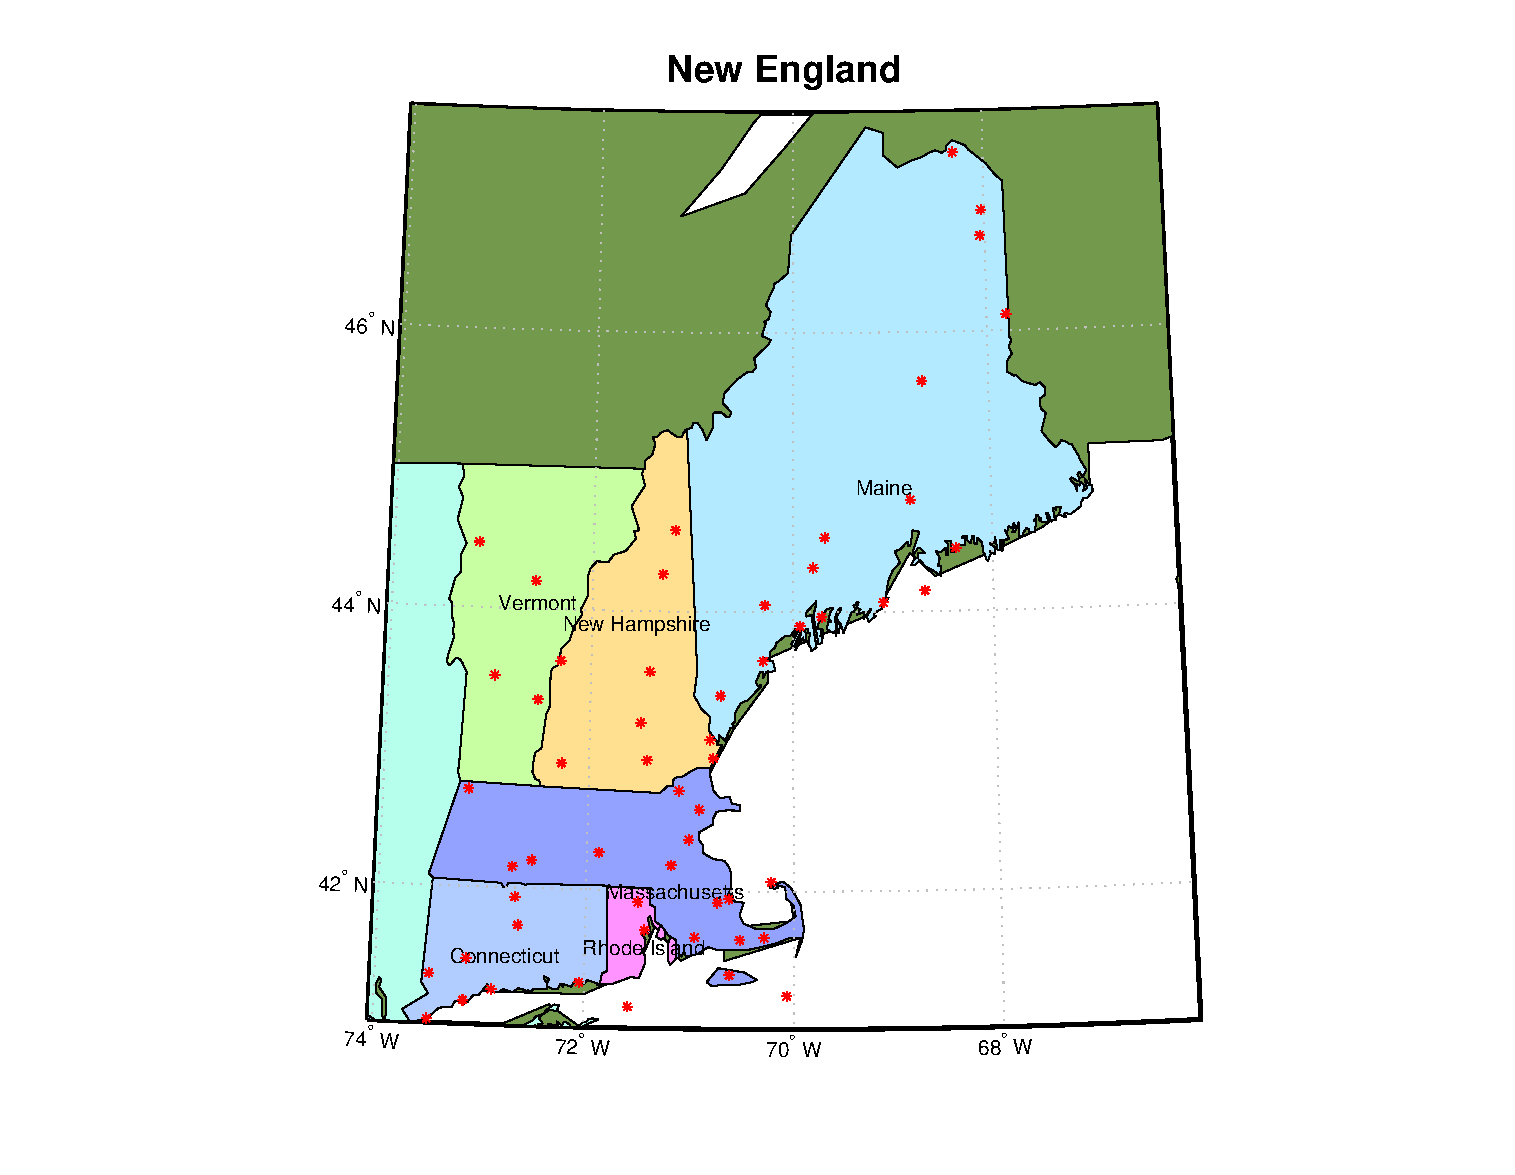
\includegraphics[width=1\columnwidth]{img/NE_map}
\caption{Candidate locations in New England}
\label{fig:NE_locs}
\end{figure}

We adopt the values and approaches for computing PUE, datacenter construction costs, wind farm construction costs, land costs, transmission lines and network connection costs, and grid energy costs from \cite{berral2014building}.  \thunote{I think we need a summary table here to give information.}

\thunote{Xiaoying, what is the assumed load?  What about the datacenter load ($powNeed$)}
For each time epoch $t$, we compute the wind energy being generated by all the wind farms (existing ones and the new one being placed) using $\beta(l,t)$.  We then compute the system loss for the time epoch for the placement of the new datacenter and wind farm at locations $d$ and $w$, respectively, using the simulation approach described in Section~\ref{sec:quantify}.  For each possible pair of ($l$, $w$), we sum the transmission loss over the entire year.

Finally, for the cost of system transmission loss, we set $priceLoss$ to the maximum electricity price in the whole area.  \thunote{Xiaoying, Divya gave us some values that we can use here.  Did we use these new values, or are we still using the maximum electricity price?}

\subsubsection{Placement approach}

To see the impact of considering transmission loss, as well as the simultaneous placement of datacenter and wind farm, we compare results for five different placement approaches:

\begin{itemize}

\item \textbf{DC\_WF\_OPT:} This strategy individually looks for the best location to put the datacenter and the wind farm; i.e., it solves the optimization problem for the datacenter without considering the new wind farm, and then solves the optimization problem again for the wind farm without considering the new datacenter.  This strategy also ignore transmission loss.

\item \textbf{DC+G\_WF+G:} This strategy is the same as DC\_WF\_OPT except that transmission loss is considered when solving the optimization problem.

\item \textbf{Min\_Loss:} This strategy finds locations for the datacenter and wind farm that minimizes the cost of transmission loss.

\item \textbf{Co-location:} This strategy assumes that the datacenter and wind farm 
should be co-located, and so finds a single location for both that minimizes the overall cost.

\item \textbf{Joint:} This strategy considers the simultaneous placement of the datacenter and wind farm, and uses all of the costs and revenues in the optimization framework.

\end{itemize}

\subsubsection{Results}
Figure \ref{fig:cost1dc1wf} shows the results of the total cost by using five different strategies when seeking the best locations when we are building a 100MW datacenter and a wind farm which can supply green energy for it.

From the figure, we can see that by considering grid costs, the total cost will be further saved compared to best choices for the datacenter and the wind farm separately. Also, $Min\_Loss$ can achieve minimal losses of all possible choices, but the total cost is large mainly because it selects an expensive place for purchasing land for the wind farm. The best choice of co-location options is also nearly 7\% higher than the $Jointly$ choice, and it's easy to understand since the best location for datacenter is not necessarily the best for wind farm and vice versa.

We calculate all of the combinations for wind farm and datacenter locations and use the average total cost of these combinations (which is \$667.1M per year) as the baseline for comparison. Then, the locations found and the corresponding cost savings of the five strategies are listed in Table \ref{tab:costsaving}.

\begin{figure}[ht]
\centering
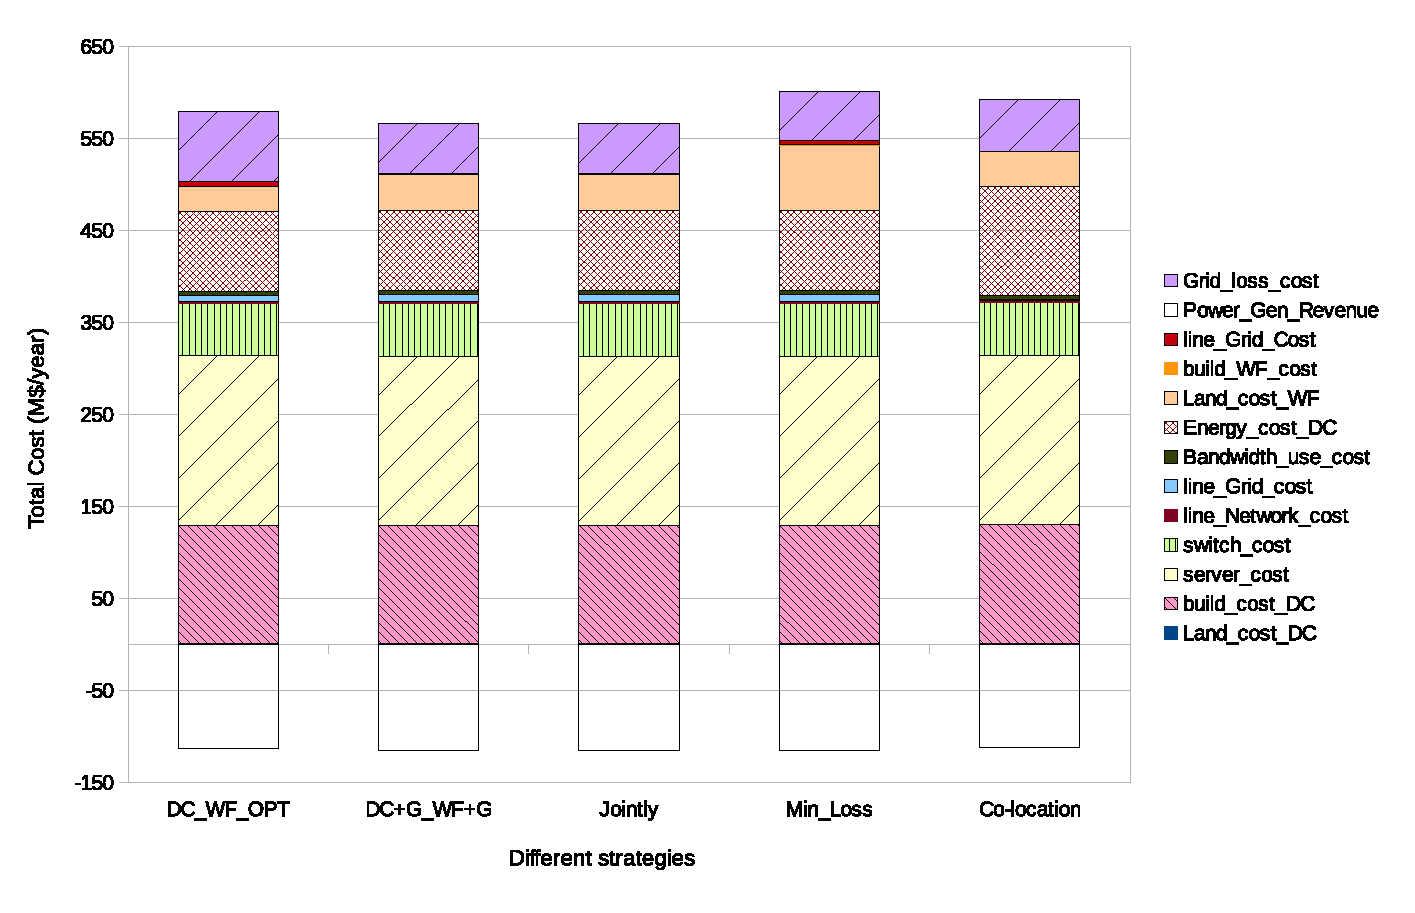
\includegraphics[width=1\columnwidth]{img/cost-one-dc-one-wf}
\caption{Costs of building one datacenter (100MW) with one wind farm}
\label{fig:cost1dc1wf}
\end{figure}

\begin{table}[ht]
\begin{center}
\caption{Detailed results of cost savings by different strategies.}
\begin{tabular}{|l|p{50pt}|p{50pt}|p{30pt}|p{20pt}|}
\hline
\textbf{Strategy}& \textbf{Datacenter location} &\textbf{Wind farm location} &\textbf{Total cost (M\$/year)} &\textbf{Cost saving (\%)} \\
\hline
\textbf{DC\_WF\_OPT} &  Burlington,NH  & Mount Washington, NH &465.6& 30.2 \\
\textbf{DC+G\_WF+G} &Springfield Hartnes, VT  & Nash Island, CO&450.3& 32.5\\
\textbf{Jointly} &Springfield Hartnes, VT&  Nash Island, CO & 450.3 & 32.5\\
\textbf{Min\_Loss} &Springfield Hartnes, VT & Marthas Vineyard, RI & 485.6& 27.2 \\
\textbf{Co-location}& Nash Island, CO &Nash Island, CO&480.7 & 27.9  \\
\hline
\end{tabular}
\label{tab:costsaving}
\end{center}
\end{table}

%%% Local Variables:
%%% mode: latex
%%% TeX-master: "paper"
%%% End:

\section{Related Work}
\label{sec:related}

This section reviews relevant work to this paper in the recent literature, which are classified into two categories.

\subsection{Datacenters participation in grid programs}

In the smart grid era, datacenters began to show the advantages for demand response and facilitate ancillary services due to its great and controllable flexibility. Researchers studied the effect of datacenter demand response on power consumption reduction \cite{lbnl12shortstudy, lbnl12report}. They found that 25\% of the demand savings can be done with minimal or no impact on datacenter performance. Also, 10\% of the load can be shed with short response time with no operational impact. They did not consider dynamic load migration of the workload which can result in further reduction in power demand. 	

Mohsenian $\textit{et al.}$ in \cite{Mohsenian-Rad10grid} proposed a request distribution policy among datacenters to ensure power load balancing. They tried to minimize the maximum power on any transmission line by distributing the computing requests to suitable datacenter. Their work assumes that a fairly large number of datacenters (e.g. 6) are connected to the same power distribution network. In practice, it is very rare for some company to build several datacenters connected to the same power distribution network.
Aikema $\textit{et al.}$ in \cite{Aikema12} studied the energy cost savings that can be achieved when datacenter participates in ancillary services. Their simulation shows that 12\% cost savings can be done at the cost of 2\% performance loss (i.e. increased latency).

Recently, Wierman $\textit{et al.}$ \cite{AdamWierman2014} surveyed the opportunities and challenges for datacenters to ease the incorporation of renewable energy source into the grid and shaving the peak load. Further, Liu $\textit{et al.}$ in \cite{liu2014pricing} focused on the impact of datacenter demand response on grid. They concluded that datacenter demand response can reduce the storage requirement of a grid with renewable energy source. The other key finding of their work is voltage violation frequency is lower when datacenter is placed on the same power bus with the PV solar source.

Different from these work, we quantify the datacenter impact on the grid by focusing on the losses brought because of penetrating additional load and generations to the grid network in a regional area. By incorporating such effects into a holistic framework, we convert such losses to grid operational costs and regard it as part of the total cost when building and planning the capacity of datacenters and also the renewable energy power plants.

\subsection{Datacenter placement and capacity planning}

Some prior work has discussed about the placement issues of datacenters. Alger \cite{Dalger05} explained how to choose an optimal location for the datacenter several years ago, by considering hazars, accessibility and scalability factors. Stansberr \cite{Stansberr06} ranked some cities by estimating the annual operation costs of the datacenter. Oley \cite{Boley09} considered looking for a proper location for the datacenter establishment only by investigating the power rates of different states.
Goiri $\textit{et al.}$ \cite{Goiri11place} focused on intelligently finding the best places for building multiple datacenters to form a network for interactive Internet services. This work is to some extent close to ours, but they didn't consider the provisioning issues of renewable energy plants and the relevant costs.

Larumbe $\textit{et al.}$ \cite{larumbe2012optimal} presented a mathematical problem aiming at solving the location and routing of cloud service components. Gao $\textit{et al.}$ \cite{gao2013answer} studied how to sit datacenters near existing wind farms, and distributing load using a greedy online algorithm.
Berral $\textit{et al.}$ \cite{berral2014building} considered to select sites for datacenters and on-site power plants aiming at follow-the renewable cloud services. Unlike our work, they didn't put insights the possible impact of datacenters and distributed energy generations on the utility grid system.
A very close paper to our work is \cite{liu2014pricing} which considered a realistic distribution system and discussed how it impacts the voltage in the distribution system, while we are focusing on the transmission system of the grid.

Different from these work, we quantify and incorporate the impact of the site selection on the grid operation, and regard the summarized cost as the objective, which shows the importance of collaborating service providers and grid operators together to do the site and capacity planning.


\section{Conclusion}
\label{sec:conclusion}

In this paper, we studied the problem of smartly placing green data centers in proper locations with considering the impact on electricity grid. Since connecting data centers and renewable energy plants to the utility grid will change the power flow of the whole grid network, and thus the grid losses should be incorporated when trying to minimize the total cost. In this context, we proposed an optimization framework with the purpose of optimizing the total cost including data center, renewable energy plant and also the grid cost. The problem is formulated with several necessary constraints according to the reliablity issues for the grid. By solving the problem, we tried to seek for best locations for sitting and provisioning the capacity of both data centers and renewable energy plants. Our optimization results show that considering the grid cost will have different impact on the placement choice for sitting data centers and renewable power plants. This means grid-aware placement stategies could further help saving the overall cost from the perspective of both IT companies and grid operators.


%\section*{Acknowledgements}
\label{sec:acks}
\red{This work has been partially supported by NSFC grant No. 61363019, NSF grant XXXXX, the Rutgers Green Computing Initiative, and
the BSC-CNS Severo Ochoa program and the TIN2012- 34557 project. }

\bibliographystyle{IEEEtran}
\bibliography{paper}

\end{document}
